\begin{center}
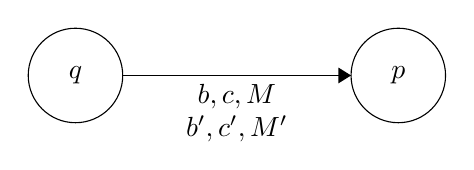
\begin{tikzpicture}[scale=0.2]
\tikzstyle{every node}+=[inner sep=0pt]
\draw [black] (11.8,-27.6) circle (3);
\draw (11.8,-27.6) node {$q$};
\draw [black] (32.3,-27.6) circle (3);
\draw (32.3,-27.6) node {$p$};
\draw [black] (14.8,-27.6) -- (29.3,-27.6);
\fill [black] (29.3,-27.6) -- (28.5,-27.1) -- (28.5,-28.1);
\draw (22.05,-28.1) node [below] {$b,c,M$};
\draw (22.05,-30.1) node [below] {$b',c',M'$};
\end{tikzpicture}
\end{center}